% generated by Plantuml 1.2025.4       
\definecolor{plantucolor0000}{RGB}{255,255,255}
\definecolor{plantucolor0001}{RGB}{0,0,0}
\definecolor{plantucolor0002}{RGB}{194,194,194}
\definecolor{plantucolor0003}{RGB}{24,24,24}
\definecolor{plantucolor0004}{RGB}{84,84,84}
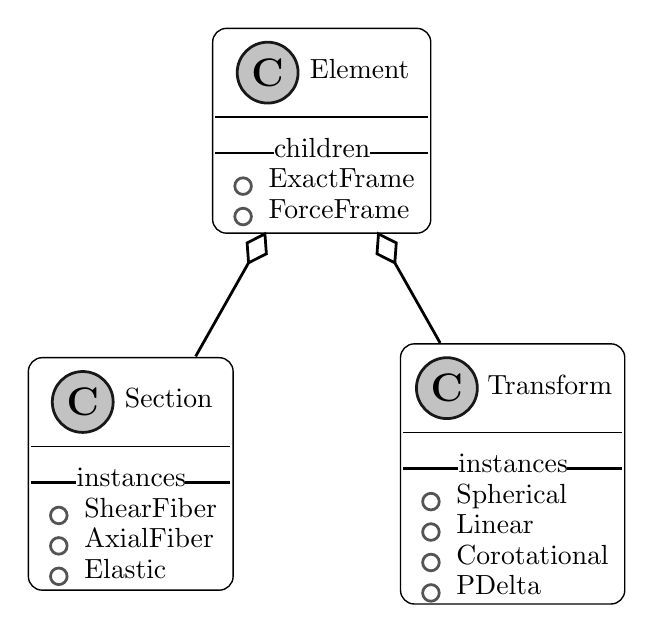
\begin{tikzpicture}[yscale=-1
,pstyle0/.style={color=black,fill=white,line width=0.5pt}
,pstyle1/.style={color=plantucolor0003,fill=plantucolor0002,line width=1.0pt}
,pstyle2/.style={color=black,line width=0.5pt}
,pstyle3/.style={color=plantucolor0004,line width=1.0pt}
,pstyle4/.style={color=black,line width=1.0pt}
]
\draw[pstyle0] (73.59pt,12pt) arc (180:270:5pt) -- (78.59pt,7pt) -- (147.4pt,7pt) arc (270:360:5pt) -- (152.4pt,12pt) -- (152.4pt,76pt) arc (0:90:5pt) -- (147.4pt,81pt) -- (78.59pt,81pt) arc (90:180:5pt) -- (73.59pt,76pt) -- cycle;
\draw[pstyle1] (93.468pt,23pt) ellipse (11pt and 11pt);
\node at (93.468pt,23pt)[]{\textbf{\Large C}};
\node at (108.552pt,18pt)[below right,color=black,inner sep=0]{Element};
\draw[pstyle2] (74.59pt,39pt) -- (151.4pt,39pt);
\draw[pstyle3] (84.59pt,64pt) ellipse (3pt and 3pt);
\node at (93.59pt,57.5pt)[below right,color=black,inner sep=0]{ExactFrame};
\draw[pstyle3] (84.59pt,75pt) ellipse (3pt and 3pt);
\node at (93.59pt,68.5pt)[below right,color=black,inner sep=0]{ForceFrame};
\draw[pstyle4] (74.59pt,52pt) -- (95.615pt,52pt);
\node at (95.615pt,46.5pt)[below right,color=black,inner sep=0]{children};
\draw[pstyle4] (130.375pt,52pt) -- (151.4pt,52pt);
\draw[pstyle0] (7pt,131pt) arc (180:270:5pt) -- (12pt,126pt) -- (75.99pt,126pt) arc (270:360:5pt) -- (80.99pt,131pt) -- (80.99pt,205pt) arc (0:90:5pt) -- (75.99pt,210pt) -- (12pt,210pt) arc (90:180:5pt) -- (7pt,205pt) -- cycle;
\draw[pstyle1] (26.644pt,142pt) ellipse (11pt and 11pt);
\node at (26.644pt,142pt)[]{\textbf{\Large C}};
\node at (41.676pt,137pt)[below right,color=black,inner sep=0]{Section};
\draw[pstyle2] (8pt,158pt) -- (79.99pt,158pt);
\draw[pstyle3] (18pt,183pt) ellipse (3pt and 3pt);
\node at (27pt,176.5pt)[below right,color=black,inner sep=0]{ShearFiber};
\draw[pstyle3] (18pt,194pt) ellipse (3pt and 3pt);
\node at (27pt,187.5pt)[below right,color=black,inner sep=0]{AxialFiber};
\draw[pstyle3] (18pt,205pt) ellipse (3pt and 3pt);
\node at (27pt,198.5pt)[below right,color=black,inner sep=0]{Elastic};
\draw[pstyle4] (8pt,171pt) -- (24.22pt,171pt);
\node at (24.22pt,165.5pt)[below right,color=black,inner sep=0]{instances};
\draw[pstyle4] (63.77pt,171pt) -- (79.99pt,171pt);
\draw[pstyle0] (141.47pt,126pt) arc (180:270:5pt) -- (146.47pt,121pt) -- (217.51pt,121pt) arc (270:360:5pt) -- (222.51pt,126pt) -- (222.51pt,210pt) arc (0:90:5pt) -- (217.51pt,215pt) -- (146.47pt,215pt) arc (90:180:5pt) -- (141.47pt,210pt) -- cycle;
\draw[pstyle1] (158.234pt,137pt) ellipse (11pt and 11pt);
\node at (158.234pt,137pt)[]{\textbf{\Large C}};
\node at (172.626pt,132pt)[below right,color=black,inner sep=0]{Transform};
\draw[pstyle2] (142.47pt,153pt) -- (221.51pt,153pt);
\draw[pstyle3] (152.47pt,178pt) ellipse (3pt and 3pt);
\node at (161.47pt,171.5pt)[below right,color=black,inner sep=0]{Spherical};
\draw[pstyle3] (152.47pt,189pt) ellipse (3pt and 3pt);
\node at (161.47pt,182.5pt)[below right,color=black,inner sep=0]{Linear};
\draw[pstyle3] (152.47pt,200pt) ellipse (3pt and 3pt);
\node at (161.47pt,193.5pt)[below right,color=black,inner sep=0]{Corotational};
\draw[pstyle3] (152.47pt,211pt) ellipse (3pt and 3pt);
\node at (161.47pt,204.5pt)[below right,color=black,inner sep=0]{PDelta};
\draw[pstyle4] (142.47pt,166pt) -- (162.215pt,166pt);
\node at (162.215pt,160.5pt)[below right,color=black,inner sep=0]{instances};
\draw[pstyle4] (201.765pt,166pt) -- (221.51pt,166pt);
\draw[pstyle4] (86.5709pt,91.7142pt) ..controls (78.7009pt,105.6242pt) and (75.58pt,111.15pt) .. (67.46pt,125.51pt);
\draw[pstyle4] (92.48pt,81.27pt) -- (86.044pt,84.5224pt) -- (86.5709pt,91.7142pt) -- (93.0068pt,88.4618pt) -- (92.48pt,81.27pt) -- cycle;
\draw[pstyle4] (139.4136pt,91.7174pt) ..controls (146.4036pt,104.0874pt) and (148.42pt,107.63pt) .. (155.79pt,120.67pt);
\draw[pstyle4] (133.51pt,81.27pt) -- (132.9793pt,88.4615pt) -- (139.4136pt,91.7174pt) -- (139.9442pt,84.5258pt) -- (133.51pt,81.27pt) -- cycle;
\end{tikzpicture}
